% fig2_energy_rate — energy rate vs load, three drone presets
% 用途: 交底书 图2, §五 载重-能耗耦合模型 (创新点2 的物理基础)
% 数据: DRONE_PRESETS (a3_python/route.py:68-90):
%   light:    alpha 0.15 Wh/m, beta 0.010 Wh/m/kg, cap 5    kg
%   standard: alpha 0.10 Wh/m, beta 0.005 Wh/m/kg, cap 50   kg
%   heavy:    alpha 0.08 Wh/m, beta 0.002 Wh/m/kg, cap 500  kg
% 模型: rho(L) = alpha + beta*L
% 编译: latexmk -pdf -xelatex fig2_energy_rate.tex
\documentclass[tikz,border=8pt]{standalone}
\usepackage{amsmath}
\usepackage{pgfplots}
\pgfplotsset{compat=1.18}
\begin{document}
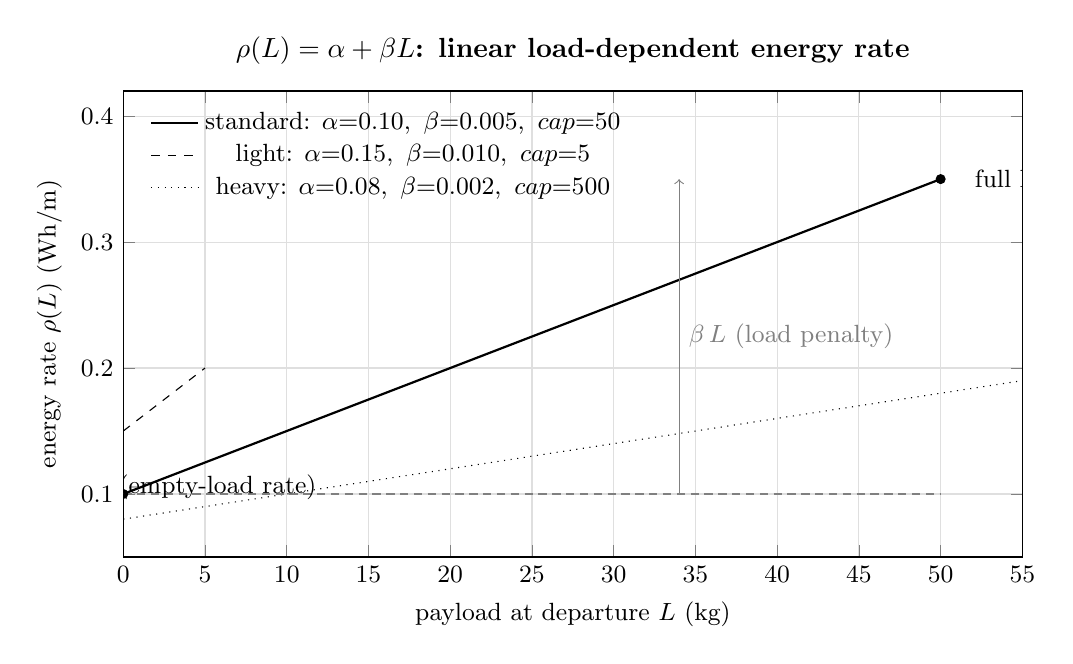
\begin{tikzpicture}
\begin{axis}[
  width=13cm, height=7.5cm,
  xlabel={payload at departure $L$ (kg)}, ylabel={energy rate $\rho(L)$ (Wh/m)},
  xmin=0, xmax=55, ymin=0.05, ymax=0.42,
  grid=both, grid style={gray!25},
  legend style={at={(0.02,0.98)},anchor=north west,draw=none,fill=none,font=\small},
  title={\textbf{$\rho(L)=\alpha+\beta L$: linear load-dependent energy rate}},
  label style={font=\small}, tick label style={font=\small},
]
% standard (baseline): alpha=0.10, beta=0.005, cap 50 -> to L=50
\addplot[thick, domain=0:50, samples=40] {0.10 + 0.005*x};
\addlegendentry{standard: $\alpha{=}0.10,\ \beta{=}0.005,\ cap{=}50$}
% light: alpha=0.15, beta=0.01, cap 5
\addplot[dashed, domain=0:5, samples=20] {0.15 + 0.01*x};
\addlegendentry{light: $\alpha{=}0.15,\ \beta{=}0.010,\ cap{=}5$}
% heavy: alpha=0.08, beta=0.002, cap 500 (show 0..55 only, slope is small)
\addplot[dotted, domain=0:55, samples=40] {0.08 + 0.002*x};
\addlegendentry{heavy: $\alpha{=}0.08,\ \beta{=}0.002,\ cap{=}500$}

% annotations: alpha intercept & full-load point for standard
\draw[densely dashed, gray] (axis cs:0,0.10) -- (axis cs:50,0.10);
\draw[->, gray] (axis cs:34,0.10) -- (axis cs:34,0.35) node[midway,right,font=\small]{$\beta\,L$ (load penalty)};
\node[font=\small] at (axis cs:5,0.105) {$\alpha$ (empty-load rate)};
\filldraw (axis cs:0,0.10) circle (1.6pt);
\filldraw (axis cs:50,0.35) circle (1.6pt);
\node[font=\small,anchor=west] at (axis cs:51.5,0.35) {full load};
\end{axis}
\end{tikzpicture}
\end{document}
